\documentclass[10pt]{article}

\usepackage{geometry}
\geometry{margin = 1in,top =0.12\paperheight, headheight=\paperheight}
\usepackage[export]{adjustbox}
\usepackage{array}
\usepackage{amsmath}
\usepackage{amsfonts}
\usepackage{fancyhdr}
\usepackage{lastpage}
\usepackage{xcolor}
\pagestyle{fancy}
\fancyhf{}
\rhead{Written Assignment, Page \thepage}
\lhead{MATH211}
\chead{
\includegraphics[width = 0.15\textwidth]{MCLogo-Bck.png}}


%\renewcommand{\footrulewidth}{0.4pt}

\usepackage{enumitem}
\usepackage{pifont}
\usepackage{graphicx}
\graphicspath{{../img}}

\newtheorem{theorem}{Theorem}
\newtheorem{exercise}{Exercise}


\newcommand{\R}{\mathbb R}
\newcommand{\e}{{\rm e}}
\newcommand{\inpr}[1]{\left\langle#1\right\rangle}
\newcommand{\norm}[1]{\lVert #1 \rVert}
\newcommand{\abs}[1]{\lvert #1 \rvert}
\newcommand{\vv}{\mathbf v}
\newcommand{\uv}{\mathbf u}

\DeclareMathOperator{\xd}{d\!}
\DeclareMathOperator{\proj}{proj}

\title{}
\date{}

\begin{document}
\noindent {\bf Problems.}
\begin{enumerate}
\item
Find the measure of the angle between the given vector and the positive $x$-axis in radian between $0$ and $2\pi$, then sketch the unit vector in the direction of the given vector.
\begin{enumerate}
\item $\inpr{-4,\ 3}$
\item $-3\mathbf i - 4\mathbf j$ 
\end{enumerate}
\clearpage
\item A hot air balloon 30 ft above the ground is tethered by three cables as shown in the diagram. If the balloon is pulling upwards with a force of 900 lb ,
what is the tension in each of the three cables? The grid lines on the ground plane are spaced 10 ft apart.
\begin{figure}[h]
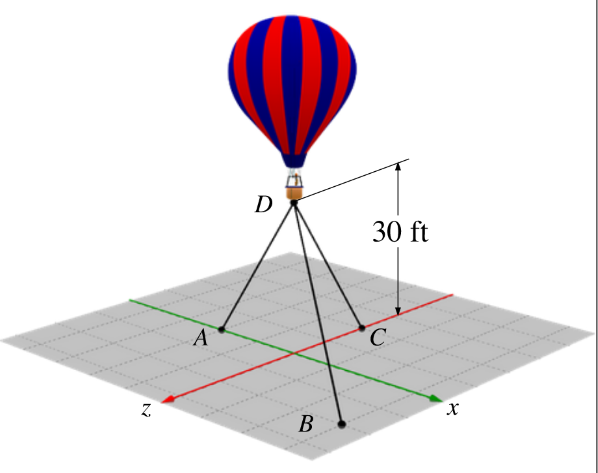
\includegraphics[width = 0.5\textwidth, right]{ballon.png}
\end{figure}
\end{enumerate}

\end{document}